\documentclass[10pt]{article}
\usepackage[utf8]{inputenc}
\usepackage[a4paper, total={6in, 8in}]{geometry}
\usepackage{graphicx}
\usepackage{longtable}

\usepackage{hyperref}
\usepackage{listings}
\usepackage[brazilian]{babel}

\font\titlefont=cmr12 at 30pt
\title{{\titlefont Análise, Projeto e Interface Humano-Computador}}

\author{\textbf{Prof.} Marcelo Medeiros Eler \\ \\ \\ Henrique Tsuyoshi Yara \textbf{NUSP:} 11796083}
\font\datafont=cmr12 at 20pt
\date{{\datafont \today}}

\begin{document}

\graphicspath{ {./images/} }


\null  % Empty line
\nointerlineskip  % No skip for prev line
\vfill
\let\snewpage \newpage
\let\newpage \relax
\maketitle
\let \newpage \snewpage
\vfill 
\break % page break
\setlength{\parindent}{5ex}
\newpage

\tableofcontents

\newpage

\section{Tarefa 1}

\subsection{Enunciado} \hfill

Avaliação de interface (individual ou em dupla)

\begin{itemize}
    \item Escolher um software (web, móvel, desktop) e fazer uma análise de sua interface:
    \begin{itemize}
        \item destacar os pontos positivos
        \item destacar os pontos negativos
    \end{itemize}
    \item Não é preciso seguir nenhum método de avaliação: usem o conhecimento, as impressões, a familiaridade e o julgamento pessoal de vocês. Não há padrão também sobre como apresentar o resultado da análise de vocês. É uma primeira atividade par começar a pensar na qualidade de interfaces e interações.
    \item Entrega em PDF, com o nome de quem fez o trabalho.
\end{itemize}

\newpage

\subsection{Apresentação do Software} \hfill

O Software escolhido foi o \textbf{KDE}. O \textbf{KDE} é um \textbf{Desktop Environment}, portanto tem a função de dar para ou usuário uma interface gráfica como: ícones, papéis de parede, widgets, barra de ferramentas, etc...

O objetivo desse software, como outros \textbf{Desktop Environments} é melhorar a experiência do usuário durante o uso do linux, para isso ele vem com várias aplicações segundárias, instaladas e tematizadas, para ajustar o som, interagir com as redes wi-fi, facilitar o manejamento das versões do kernel do linux, etc...

Como o \textbf{Desktop Environment} é um conjunto de aplicações, foram escolhidos alguns aplicativos principais que servem para configurar o sistema ou o \textbf{Desktop Environment} em si.

Nessa tarefa vão ser analisadas a \textbf{tela inicial}, o \textbf{menu} e o \textbf{menu de configurações}.

\begin{enumerate}
    \item \textbf{Tela inicial}
    \begin{figure}[h]
        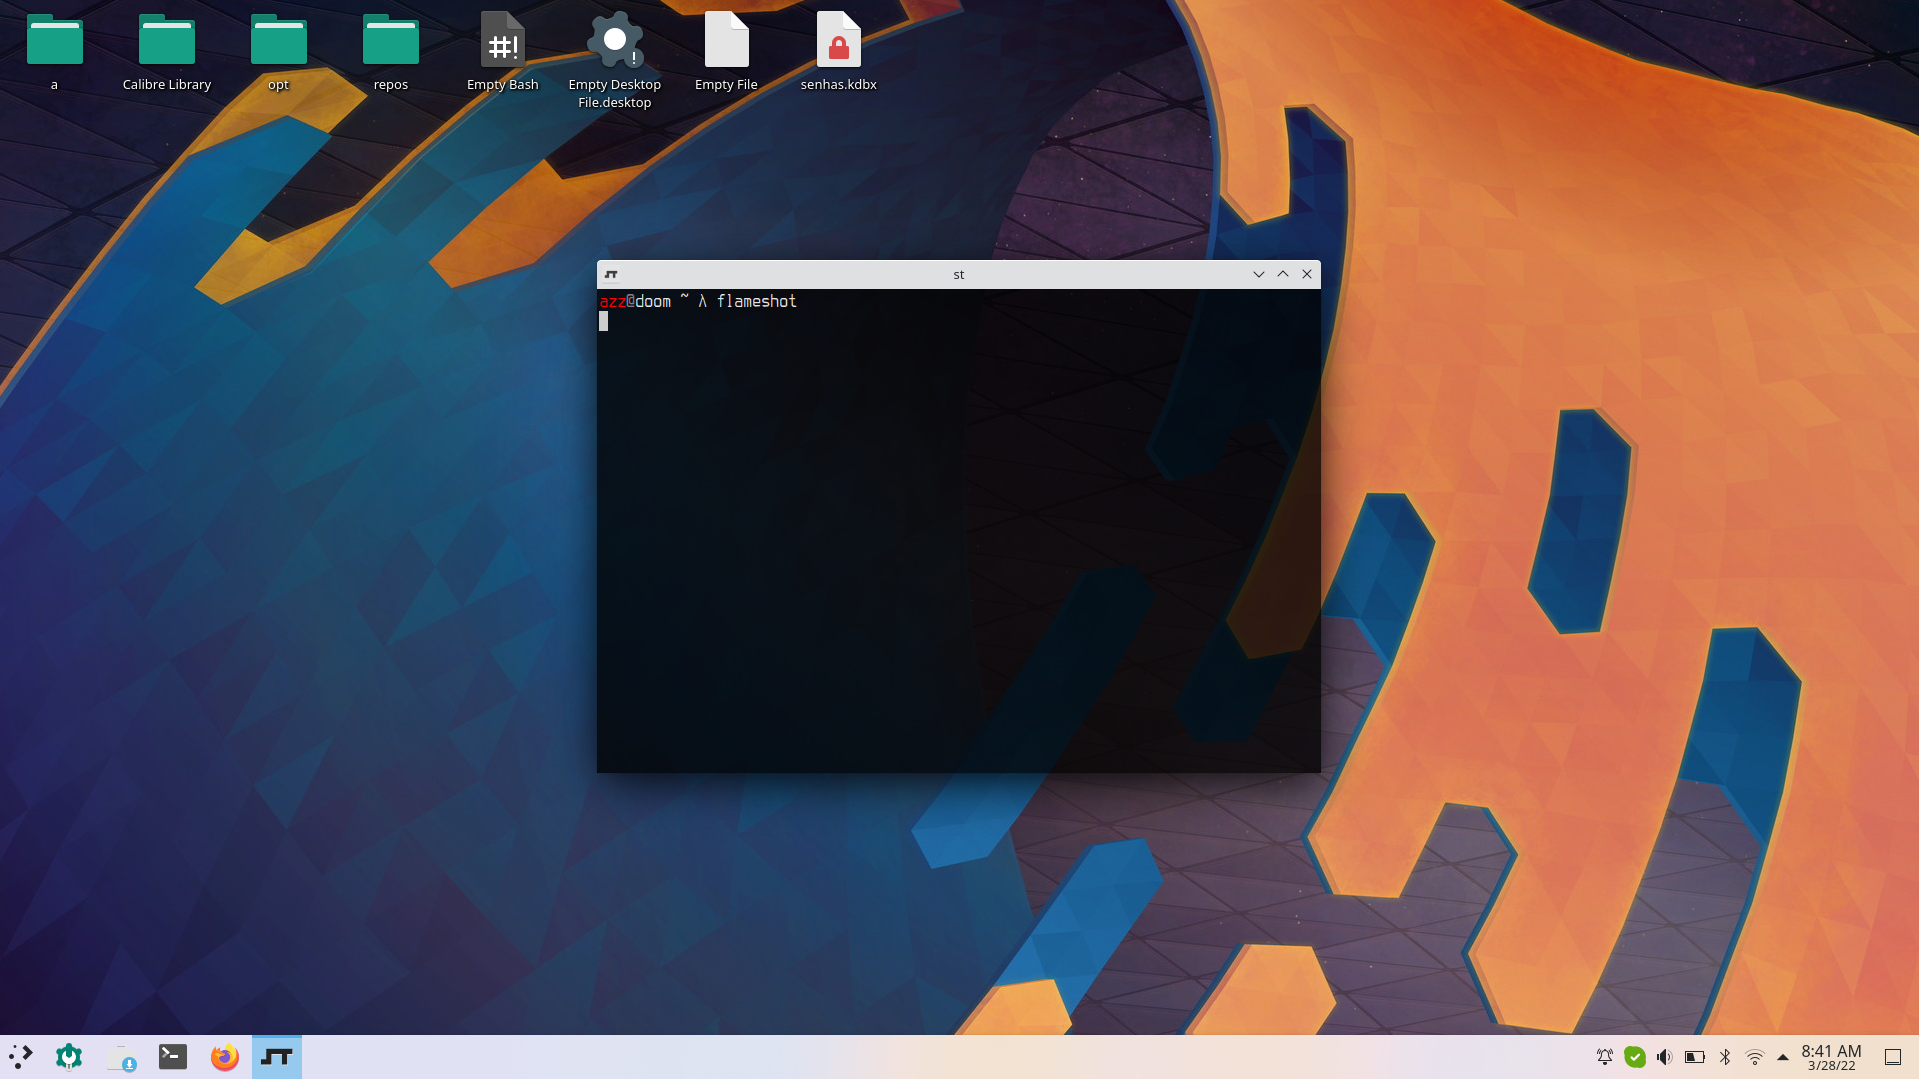
\includegraphics[width=16cm]{desktop}
        \centering
    \end{figure}
    \newpage
    \item \textbf{Menu}
    \begin{figure}[h]
        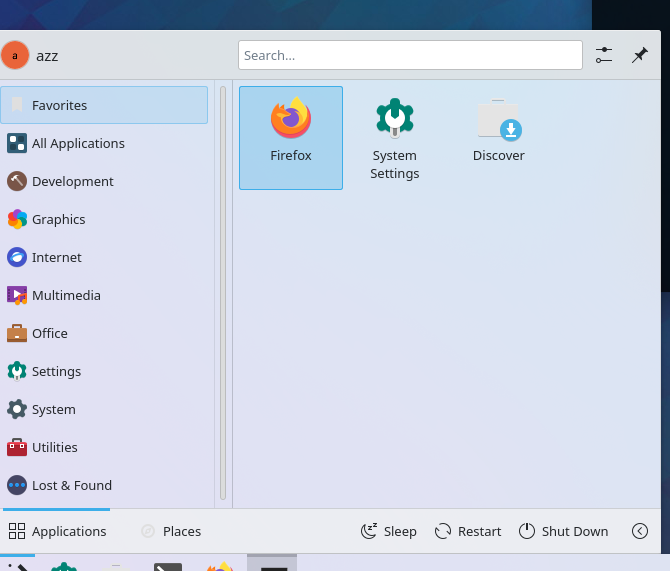
\includegraphics[width=16cm]{menu_bar}
        \centering
    \end{figure}
    \newpage
    \item \textbf{Menu de configurações}
    \begin{figure}[h]
        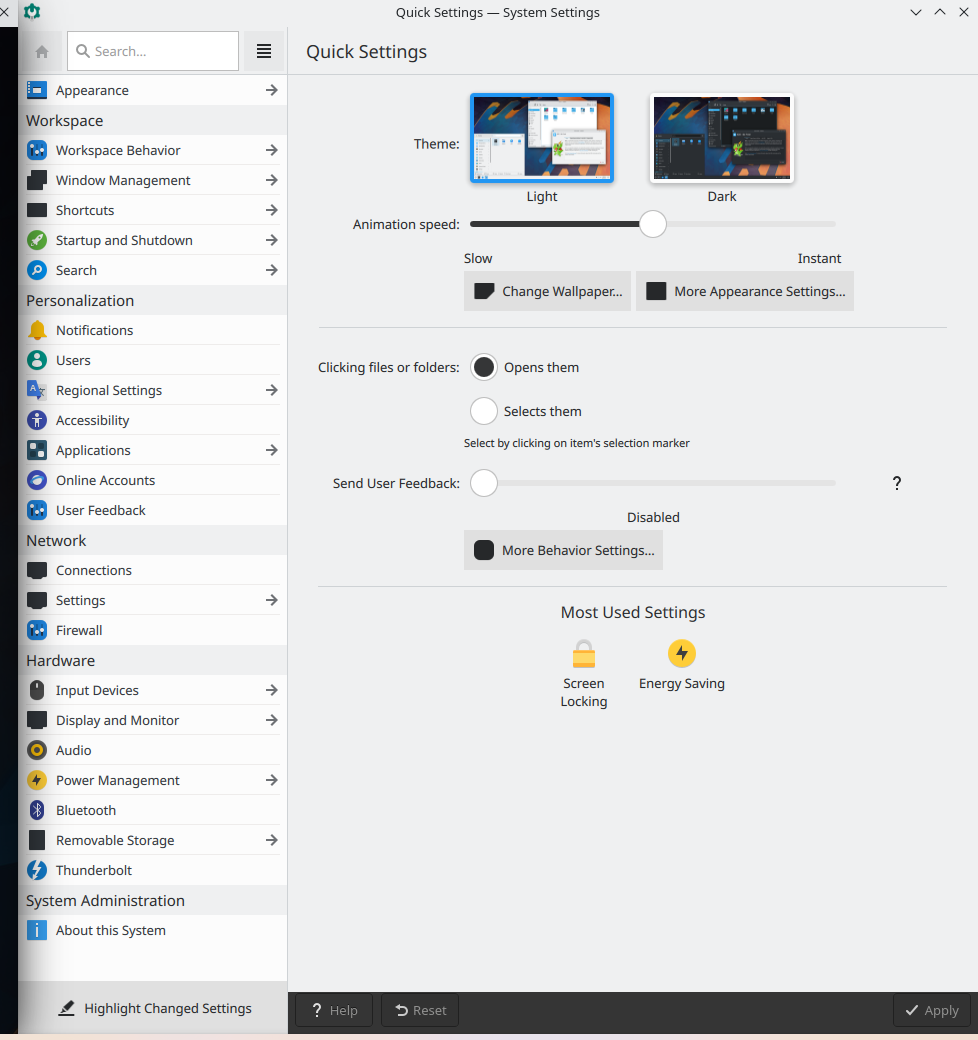
\includegraphics[width=14cm]{settings}
        \centering
    \end{figure}
\end{enumerate}

\subsection{Pontos Positivos} \hfill

\begin{itemize}
    \item Desktop:
    \begin{itemize}
        \item É possível perceber que o \textbf{KDE} coloca na barra inferior direita o aplicativo \textbf{skype} que estava rodando em plano de fundo
        \item Além disso ele deixa algumas ferramentas de configuração que são usadas no dia-a-dia na barra inferior direita, alguns exemplos disso são: notificações, interface de áudio, interface bluetooth, interface de redes, relógio, entre outros
        \item Na barra inferior esquerda podemos ver alguns dos aplicativos principais que são usados no \textbf{KDE}
    \end{itemize}
    \item Barra de menu:
    \begin{itemize}
        \item É possível ver no canto superior esquedo qual usuário está usando o computador
        \item Na esquerda é possível ver algumas categorias de aplicações feitas pelo \textbf{KDE}
        \item No canto inferior direito é possível ver as opções: suspender, reiniciar e desligar
        \item No canto superior esquerdo é possível ver uma barra de pesquisa para pesquisar por applicações
    \end{itemize}
    \item Configurações:
    \begin{itemize}
        \item Nas configurações podemos ver uma barra na lateral esquerda, nela é possível ver categorias de aplicações para configurar o sistema. As categorias são: Aparência, Personalização, Redes, Hardware e Administração de sistema
        \item Na direita é possível ver alguns temas disponibilizados pelo KDE para configurar a aparência do sistema como \textbf{Light} e \textbf{Dark}
        \item Na direita também é possível ver as configurações mais utilizadas, facilitando assim o acesso de configuraçoes que são usadas frequentemente pelo usuário
    \end{itemize}
\end{itemize}

\subsection{Pontos Negativos} \hfill

Sobre a funcionalidade não tenho muito o que complementar, já que ele é bem completo.

\begin{itemize}
    \item Configurações:
    \begin{itemize}
        \item Não existem ícones únicos para: \textbf{User Feedback}, \textbf{Connections}, \textbf{Settings}, \textbf{Firewall}
        \item O ícone do \textbf{Startup and Shutdown} não é muito intuitivo
        \item A barra inferior direita ficou parecendo deslocada em relação ao software que tem um tema branco
    \end{itemize}
\end{itemize}

\end{document}
